\documentclass[unicode,11pt,a4paper,oneside,numbers=endperiod,openany]{scrartcl}

\usepackage{graphicx}
\usepackage{float}
\usepackage{mathtools}
\usepackage{amsmath}
\usepackage{booktabs}
\usepackage{siunitx}
\usepackage{listings}

\renewcommand{\thesubsection}{\arabic{subsection}}

\input{assignment.sty}


\begin{document}


\setassignment
\setduedate{Wednesday, December 20, 2023, 11:59 PM}

\serieheader{Numerical Computing}{2023}{Student: Jeferson Morales Mariciano}
{Discussed with: Martin Lettry}
{Solution for Project 5}{}
\newline

\assignmentpolicy


The purpose of this project is to implement the Simplex Method to find the solution of linear programs, involving both the minimisation and the maximisation of the objective function.

\section{Graphical Solution of Linear Programming Problems [20 points]}
Please consider the following two problems:
\begin{enumerate}
	\item[(1)] \begin{equation*}
			\begin{aligned}
				 & \text{min}  & z = 4x  & + y     \\
				 & \text{s.t.} & x + 2y  & \leq 40 \\
				 &             & x + y   & \geq 30 \\
				 &             & 2x + 3y & \geq 72 \\
				 &             & x, y    & \geq 0  \\
			\end{aligned}
		\end{equation*}
	\item[(2)] A tailor plans to sell two types of trousers, with production costs of 25 CHF and 40 CHF, respectively. The former type can be sold for 85 CHF, while the latter for 110 CHF. The tailor estimates a total monthly demand of 265 trousers. Find the number of units of each type of trousers that should be produced in order to maximise the net profit of the tailor, if we assume that the he cannot spend more than 7000 CHF in raw materials.
\end{enumerate}
Start by writing problem (2) as a linear programming problem. Then complete the following tasks:
\begin{itemize}
	\item Solve the system of inequalities.
	\item Plot the feasible region identified by the constraints.
	\item Find the optimal solution and the value of the objective function in that point.
\end{itemize}


\vspace{0.5cm}
\textbf{(1)}
Solving the system of inequalities:
\begin{equation*}
	\begin{cases}
		x + 2y  \leq 40 \\
		x + y   \geq 30 \\
		2x + 3y \geq 72 \\
		x, y \geq 0     \\
	\end{cases}
	\Rightarrow
	\begin{cases}
		r_1 : y \leq 20 - \frac{1}{2} x \\
		r_2 : y \geq 30 - x             \\
		r_3 : y \geq 24 - \frac{2}{3} x \\
		x, y \geq0                      \\
	\end{cases}
\end{equation*}

\begin{figure}[H]
	\centering
	\caption{Exercise 1.1 - Feasible Region}
	\label{fig:ex1-1}
	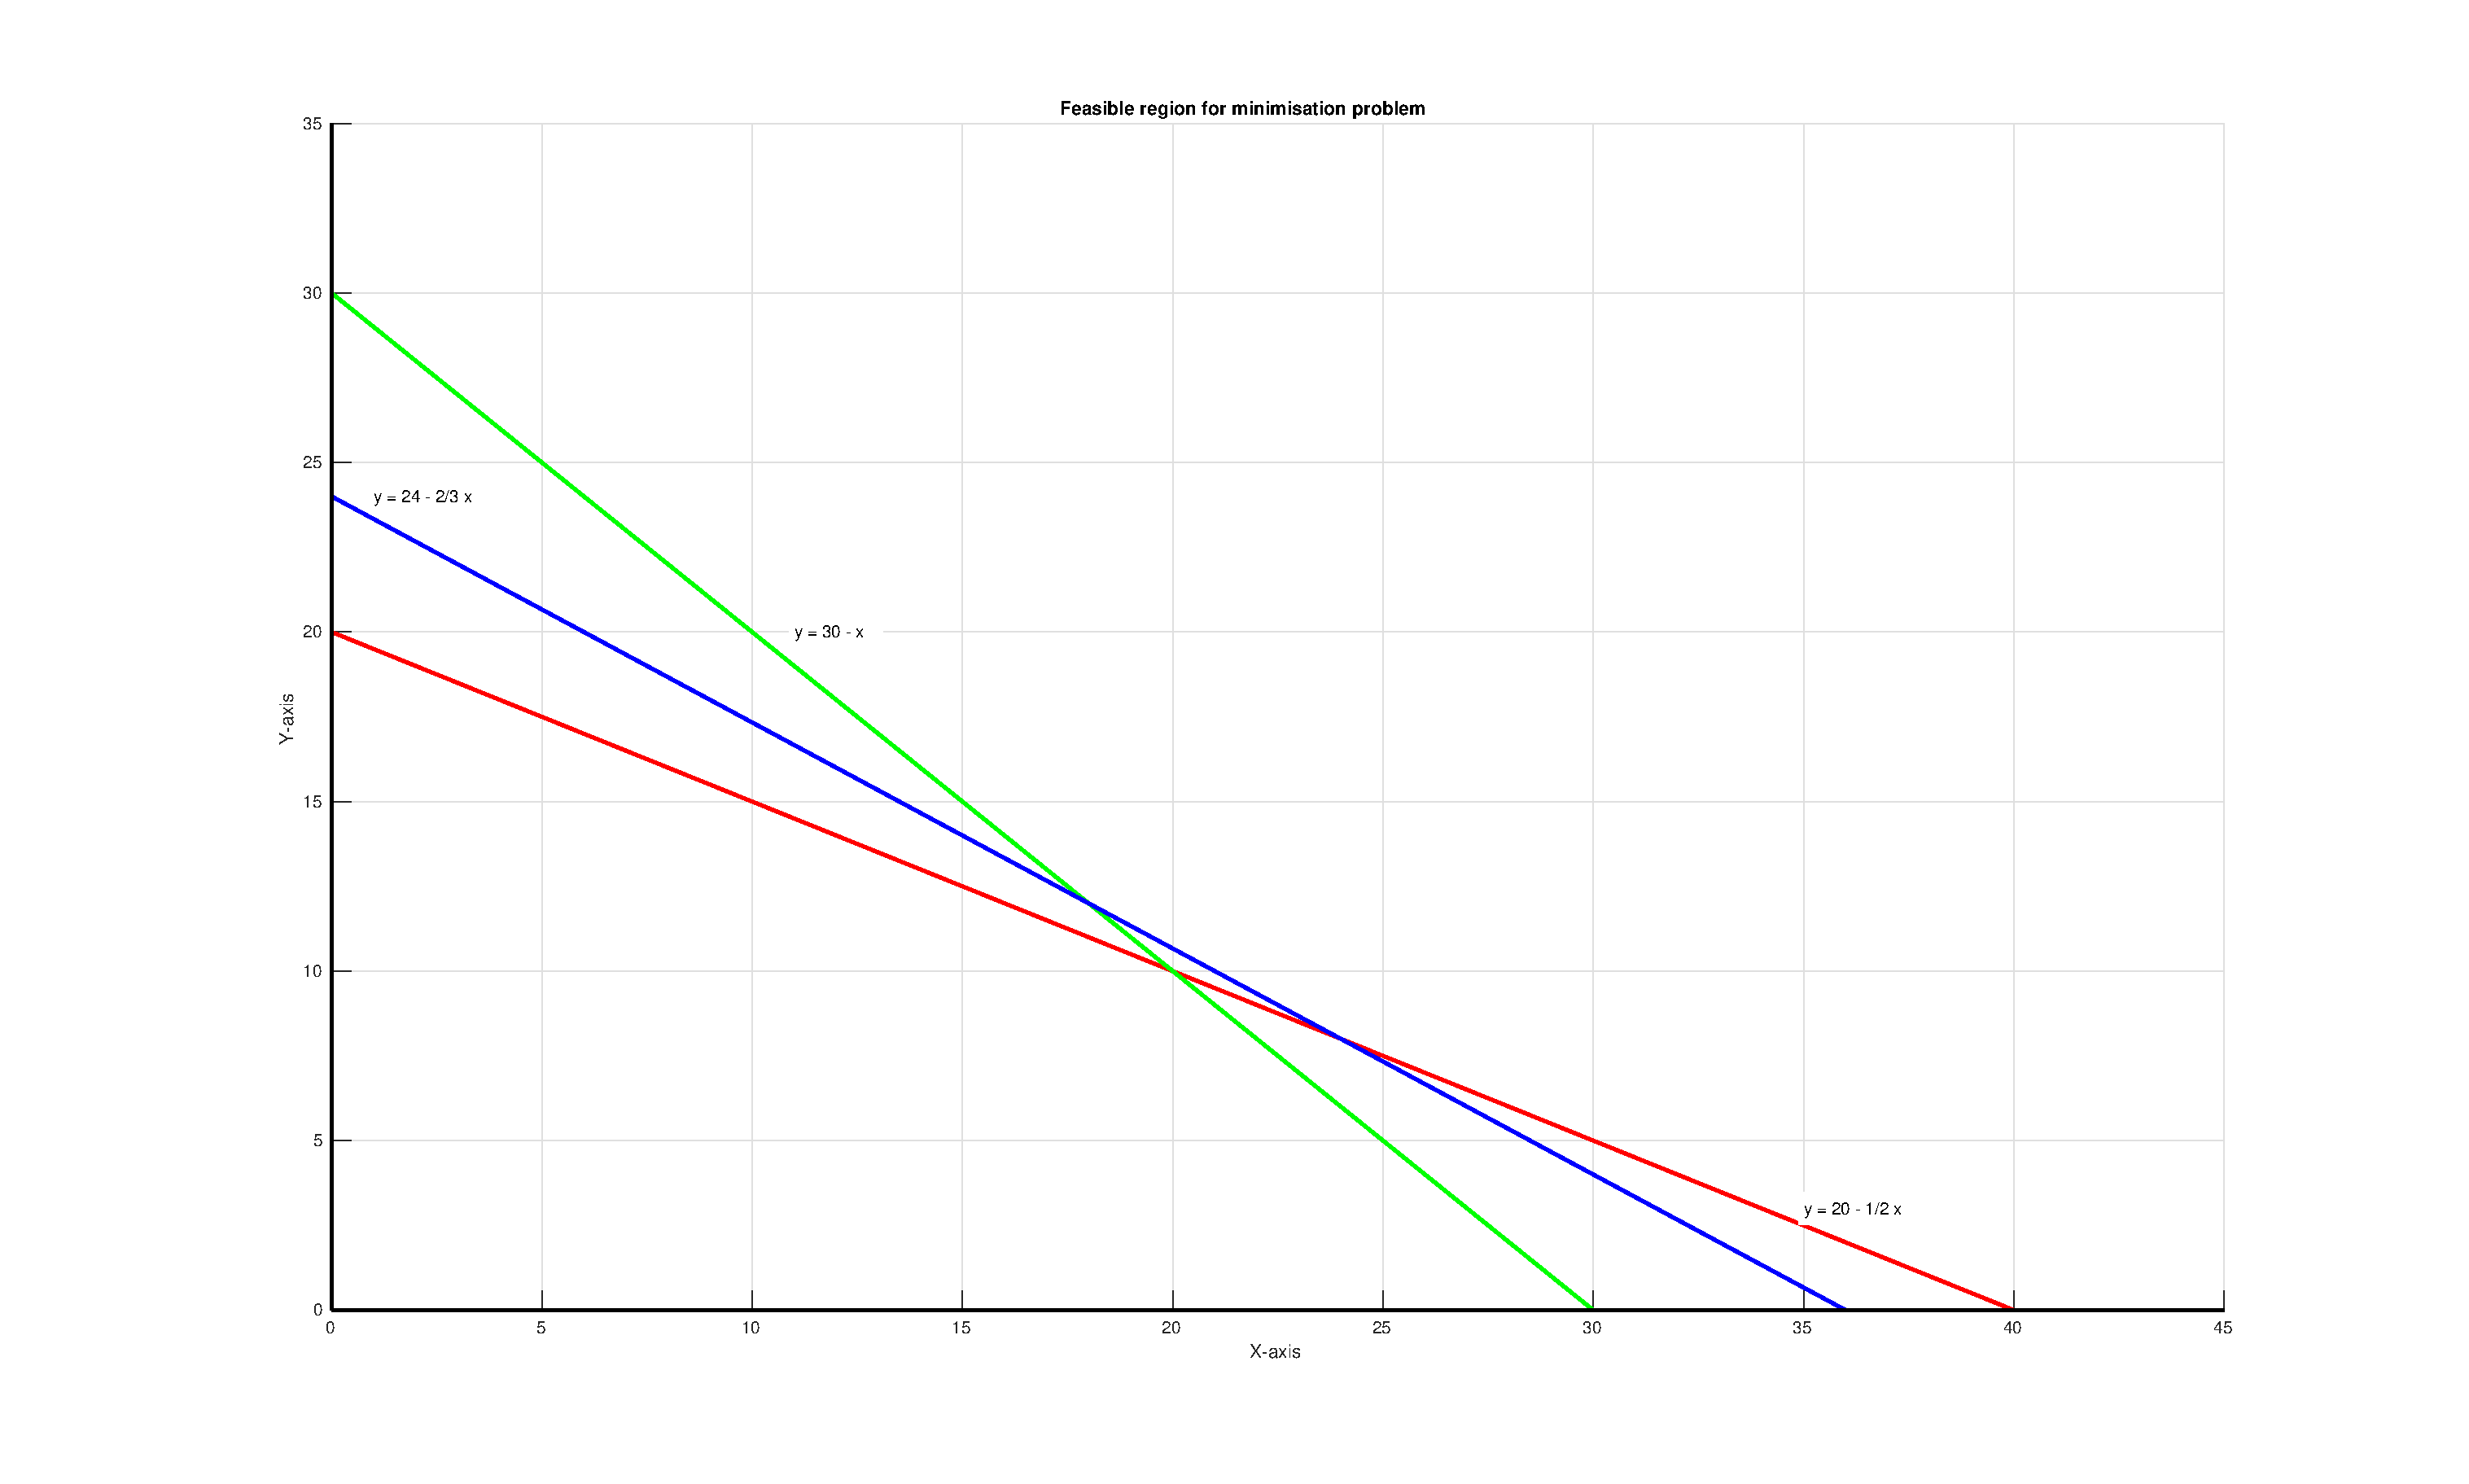
\includegraphics[width=\textwidth, trim={0cm 0cm 0cm 0cm}]{./figures/ex1-1.eps}
\end{figure}

\begin{figure}[H]
	\centering
	\caption{Exercise 1.1 - Feasible Region visualization}
	\label{fig:ex1-1-geogebra}
	\includegraphics[width=\textwidth, trim={35cm 11cm 33cm 20cm}, clip]{./figures/ex1-1-geogebra.png}
\end{figure}

The figure \ref{fig:ex1-1} shows the feasible region of the problem (1):
the 3 main lines and the non-negativity constraints in black corresponding to the x,y axis.
The figure \ref{fig:ex1-1-geogebra} shows the same feasible region,
but marking their regions with their corresponding colors to clearly see the common area overlapping.\\

To get the points of the feasible region, we can solve the system of equations:\\

Intersections at $x=0$:
\begin{equation*}
	\begin{cases}
		x \cap r_1 \\
		x \cap r_2 \\
		x \cap r_3 \\
	\end{cases}
	\Rightarrow
	\begin{cases}
		y \leq 20 - \frac{1}{2} \cdot 0 \\
		y \geq 30 - 0                   \\
		y \geq 24 - \frac{2}{3} \cdot 0 \\
	\end{cases}
	\Rightarrow
	\begin{cases}
		P_1 = (0, 20) \\
		P_2 = (0, 30) \\
		P_3 = (0, 24) \\
	\end{cases}
\end{equation*}

Intersections at $y=0$:
\begin{equation*}
	\begin{cases}
		y \cap r_1 \\
		y \cap r_2 \\
		y \cap r_3 \\
	\end{cases}
	\Rightarrow
	\begin{cases}
		0 \leq 20 - \frac{1}{2} x \\
		0 \geq 30 - x             \\
		0 \geq 24 - \frac{2}{3} x \\
	\end{cases}
	\Rightarrow
	\begin{cases}
		P_4 = (40, 0) \\
		P_5 = (30, 0) \\
		P_6 = (36, 0) \\
	\end{cases}
\end{equation*}

Intersections between lines:
\begin{equation*}
	\begin{cases}
		r_1 \cap r_2 \\
		r_1 \cap r_3 \\
		r_2 \cap r_3 \\
	\end{cases}
	\Rightarrow
	\begin{cases}
		20 - \frac{1}{2} x = 30 - x             \\
		20 - \frac{1}{2} x = 24 - \frac{2}{3} x \\
		30 - x = 24 - \frac{2}{3} x             \\
	\end{cases}
	\Rightarrow
	\begin{cases}
		P_7 = (20, 10) \\
		P_8 = (24, 8)  \\
		P_9 = (18, 12) \\
	\end{cases}
\end{equation*}

These 3 points constitute the feasible region
because included in the regions of all constraints:

\vspace{0.5cm}
\begin{minipage}{0.4\textwidth}
	\begin{itemize}
		\setlength\itemsep{0.5em}
		\item $P_4 = (40, 0)$
		\item $P_6 = (36, 0)$
		\item $P_8 = (24, 8)$
	\end{itemize}
\end{minipage}
\begin{minipage}{0.2\textwidth}
	$\xrightarrow{\text{evaluate in z}}$
\end{minipage}
\begin{minipage}{0.4\textwidth}
	\begin{itemize}
		\setlength\itemsep{0.5em}
		\item $z(P_4) = 4 \cdot 40 + 0 = 160$
		\item $z(P_6) = 4 \cdot 36 + 0 = 144$
		\item $z(P_8) = 4 \cdot 24 + 8 = 104$
	\end{itemize}
\end{minipage}
\vspace{0.5cm}

The optimal solution is $P_8$,
with the value of the objective function $z$ minimizing the problem.

\vspace{0.5cm}
\textbf{(2)}
Rewrite the exercise as a linear programming problem:\\

\begin{minipage}{0.4\textwidth}
	\begin{itemize}
		\setlength\itemsep{0.0em}
		\item trouses type 1, 2
		\item production cost 25, 40
		\item selling price 85, 110
		\item total demand 265
		\item maximize profit
		\item spend less than 7000 in materials
	\end{itemize}
\end{minipage}
\begin{minipage}{0.2\textwidth}
	$\xrightarrow{\text{max problem}}$
\end{minipage}
\fbox{
	\begin{minipage}{0.3\textwidth}
		\begin{equation*}
			\begin{aligned}
				 & \text{max}  & z = 60 x    & + 70 y    \\
				 & \text{s.t.} & 25 x + 40 y & \leq 7000 \\
				 &             & x + y       & \leq 265  \\
				 &             & x, y        & \geq 0    \\
			\end{aligned}
		\end{equation*}
	\end{minipage}
}
\vspace{0.5cm}

Solving the system of inequalities:

\begin{equation*}
	\begin{cases}
		25 x + 40 y \leq 7000 \\
		x + y       \leq 265  \\
		x, y        \geq 0    \\
	\end{cases}
	\Rightarrow
	\begin{cases}
		r_1 : y \leq 175 - \frac{5}{8} x \\
		r_2 : y \leq 265 - x             \\
		x, y \geq 0                      \\
	\end{cases}
\end{equation*}

\begin{figure}[H]
	\centering
	\caption{Exercise 1.2 - Feasible Region}
	\label{fig:ex1-2}
	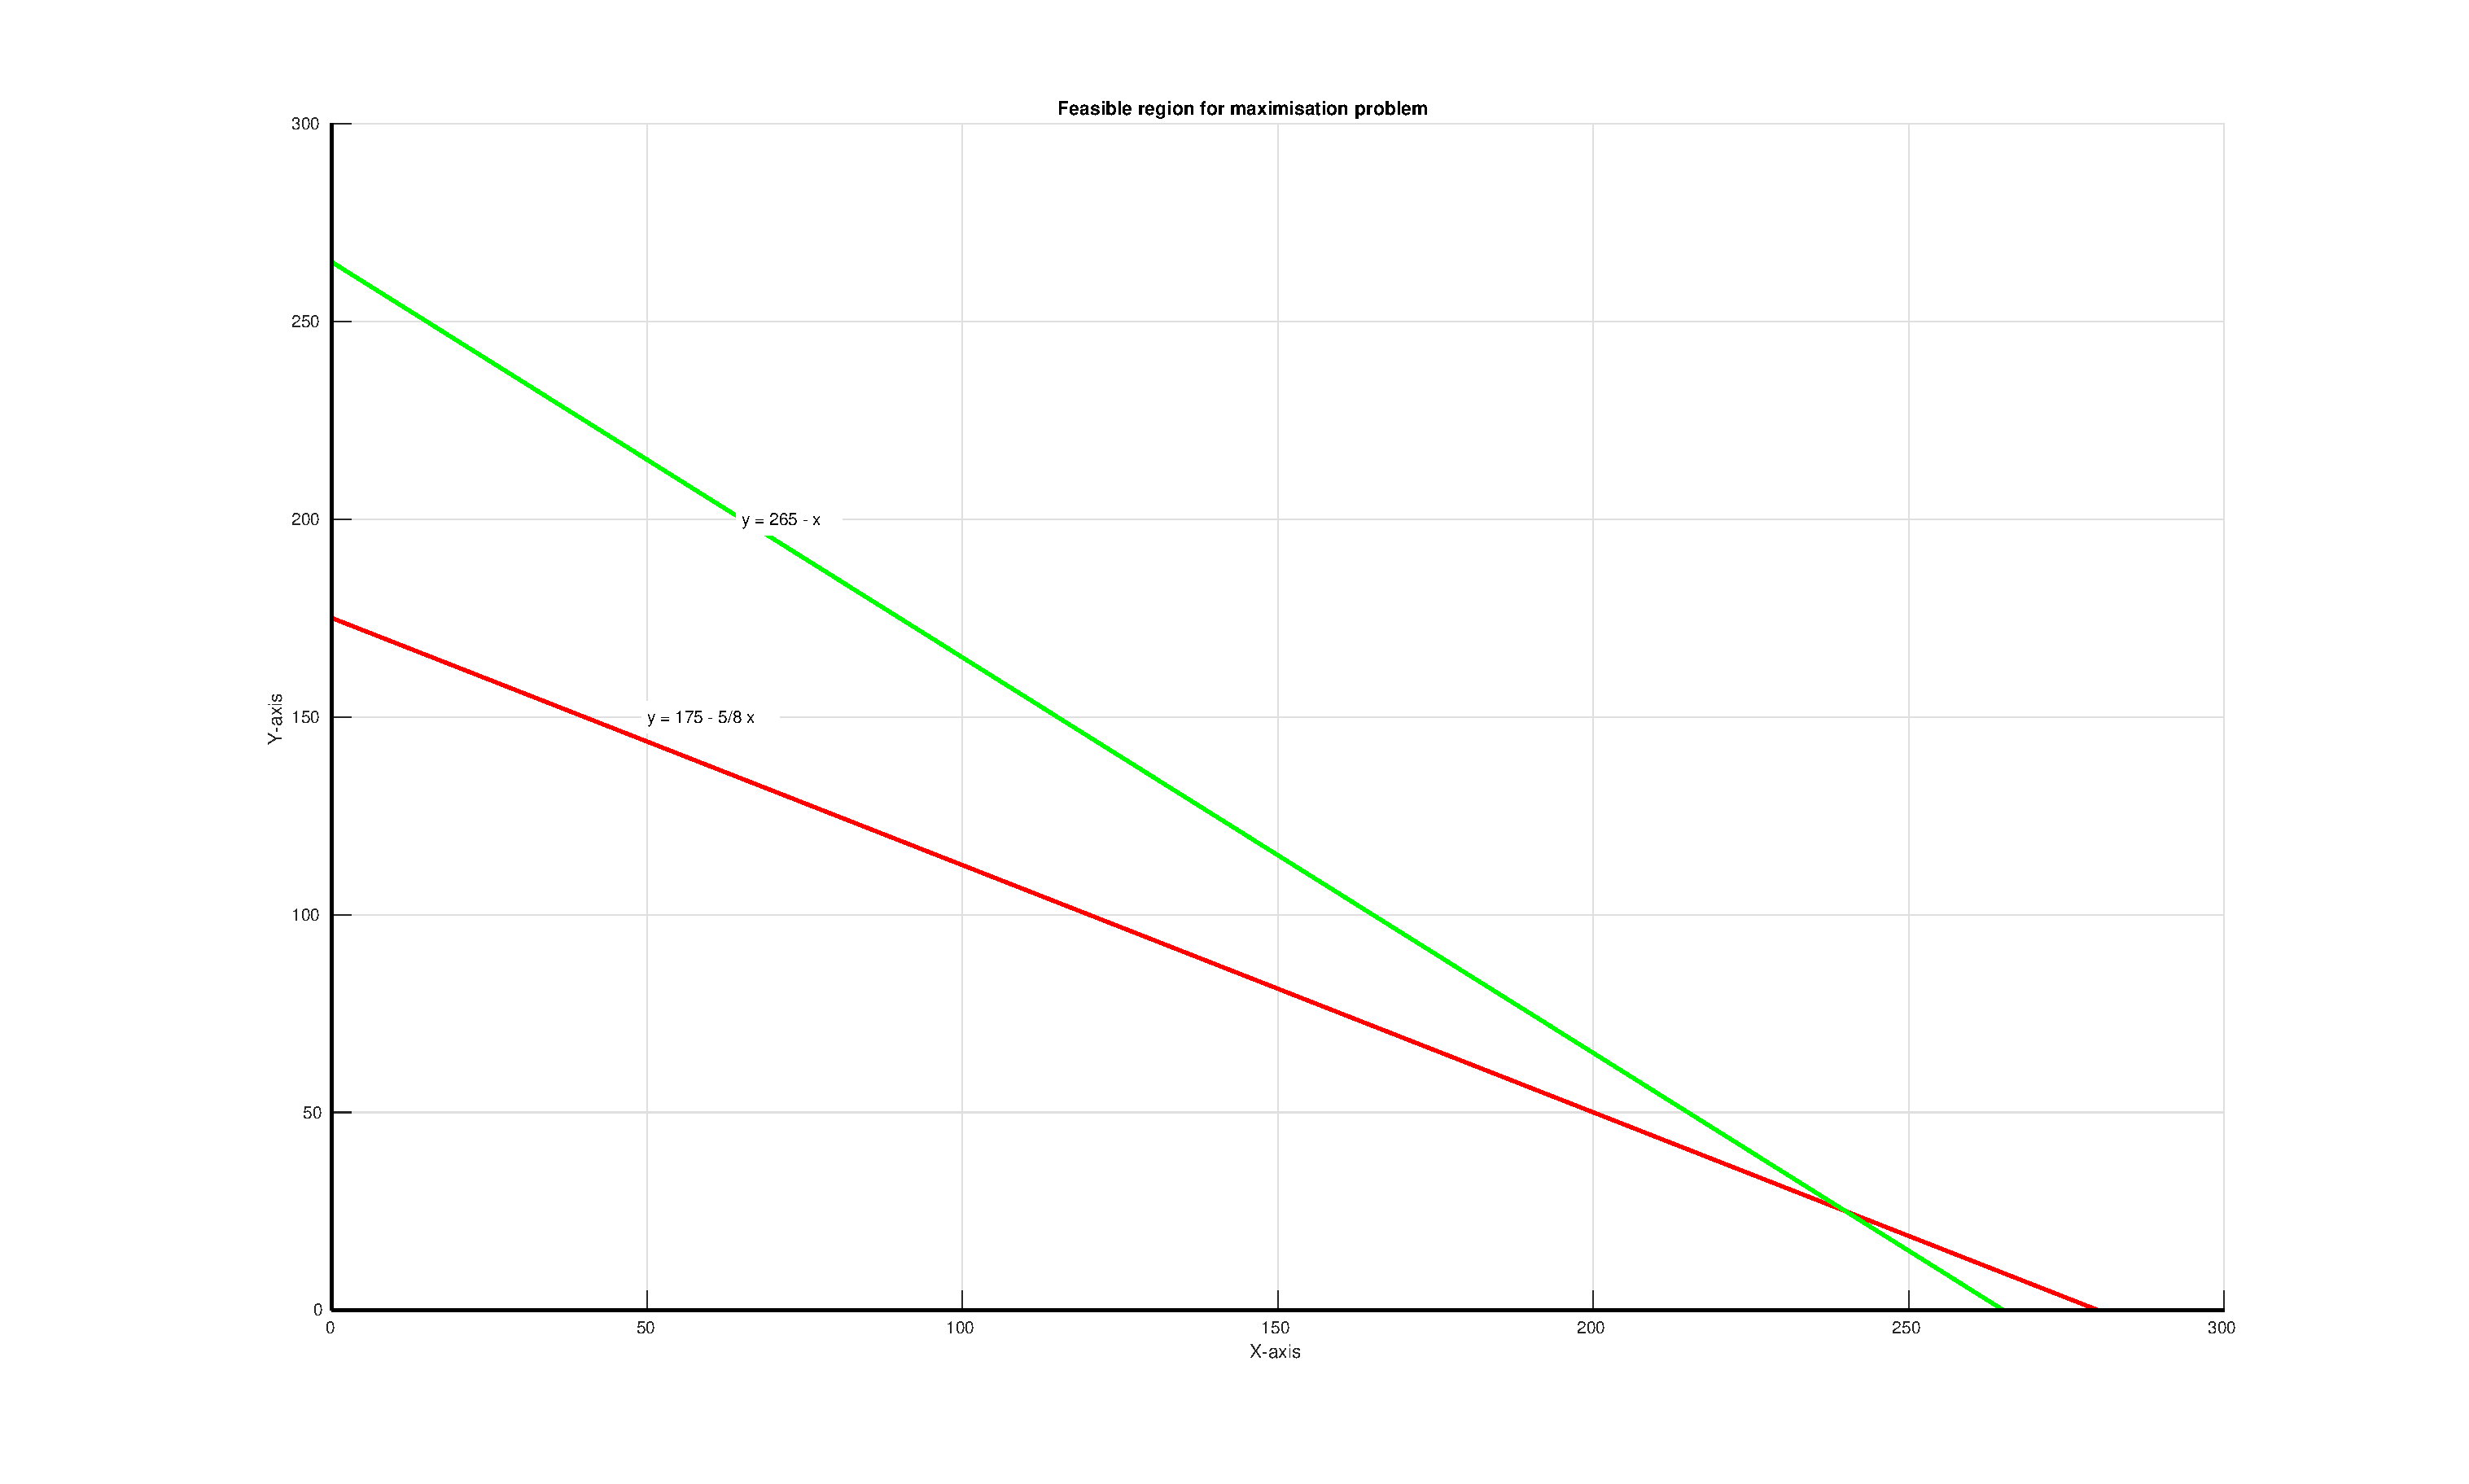
\includegraphics[width=\textwidth, trim={5cm 0cm 4cm 0cm}, clip]{./figures/ex1-2.eps}
\end{figure}

\begin{figure}[H]
	\centering
	\caption{Exercise 1.2 - Feasible Region visualization}
	\label{fig:ex1-2-geogebra}
	\includegraphics[width=\textwidth, trim={110cm 25cm 75cm 20cm}, clip]{./figures/ex1-2-geogebra.png}
\end{figure}

The figure \ref{fig:ex1-2} shows the feasible region of the problem (2):
the 2 main lines and the non-negativity constraints in black corresponding to the x,y axis
as in the previous exercise.
The figure \ref{fig:ex1-2-geogebra} shows the same feasible region,
but marking their regions with their corresponding colors red and green
to clearly see the common area overlapping in orange.\\

To get the points of the feasible region, solve the system of equations:\\

Intersections at $x=0$:
\begin{equation*}
	\begin{cases}
		x \cap r_1 \\
		x \cap r_2 \\
	\end{cases}
	\Rightarrow
	\begin{cases}
		y \leq 175 - \frac{5}{8} \cdot 0 \\
		y \geq 265 - x                   \\
	\end{cases}
	\Rightarrow
	\begin{cases}
		P_1 = (0, 175) \\
		P_2 = (0, 265) \\
	\end{cases}
\end{equation*}

Intersections at $y=0$:
\begin{equation*}
	\begin{cases}
		y \cap r_1 \\
		y \cap r_2 \\
	\end{cases}
	\Rightarrow
	\begin{cases}
		0 \leq 175 - \frac{5}{8} x \\
		0 \geq 265 - x             \\
	\end{cases}
	\Rightarrow
	\begin{cases}
		P_3 = (280, 0) \\
		P_4 = (265, 0) \\
	\end{cases}
\end{equation*}

Intersections between lines:
\begin{equation*}
	\begin{cases}
		r_1 \cap r_2 \\
	\end{cases}
	\Rightarrow
	\begin{cases}
		175 - \frac{5}{8} x = 265 - x \\
	\end{cases}
	\Rightarrow
	\begin{cases}
		P_5 = (240, 25) \\
	\end{cases}
\end{equation*}

These 3 points constitute the feasible region
because included in the regions of all constraints:

\vspace{0.5cm}
\begin{minipage}{0.3\textwidth}
	\begin{itemize}
		\setlength\itemsep{0.5em}
		\item $P_1 = (0, 175)$
		\item $P_4 = (265, 0)$
		\item $P_5 = (240, 25)$
	\end{itemize}
\end{minipage}
\begin{minipage}{0.2\textwidth}
	$\xrightarrow{\text{evaluate in z}}$
\end{minipage}
\begin{minipage}{0.5\textwidth}
	\begin{itemize}
		\setlength\itemsep{0.5em}
		\item $z(P_1) = 60 \cdot 0 + 70 \cdot 175 = 12 250$
		\item $z(P_4) = 60 \cdot 265 + 70 \cdot 0 = 15 900$
		\item $z(P_5) = 60 \cdot 240 + 70 \cdot 25 = 16 150$
	\end{itemize}
\end{minipage}
\vspace{0.5cm}

The optimal solution is $P_5$,
with the value of the objective function $z$ maximizing the net profit.

\vspace{0.5cm}

\section{Implementation of the Simplex Method [30 points]}

In this first part of the assignment, you are required to complete 2 functions which are part of a dummy implementation of the simplex method. Specifically you have to complete the TODOs in:
\begin{itemize}
	\item \emph{standardise.m}, which writes a maximisation or minimisation input problem in standard form;
	\item \emph{simplexSolve.m}, which solves a maximisation or minimisation problem using the simplex method.
\end{itemize}
You are given also some already-implemented functions to help you in your task: \emph{simplex.m} is a wrapper which calls all the functions necessary to find a solution to the linear program; \emph{auxiliary.m} solves the auxiliary problem to find a feasible starting basic solution of the linear program; \emph{printSol.m} is a function which prints the optimal solution found by the simplex algorithm. Finally, \emph{testSimplex.m} presents a series of 6 problems to check if your implementation is correct, before moving to the next part of the assignment. Additional details to aid you in your implementation can be found in the comments inside the code.

\vspace{0.5cm}\noindent
The source code of the required files has been completed and extensively commented in Matlab.

\section{Applications to Real-Life Example: Cargo Aircraft [25 points]}

In this second part of the assignment, you are required to use the simplex method implementation to solve a real-life problem taken from economics (constrained profit maximisation).

A cargo aircraft has 4 compartments (indicated simply as $S_1,\dots,S_4$) used to store the goods to be transported. Details about the weight capacity and storage capacity of the different compartments can be inferred from the data reported in the following table:

\begin{center}
	\begin{tabular}{||c | c | c ||}
		\hline
		Compartment & Weight Capacity ($t$) & Storage Capacity ($m^3$) \\ [0.5ex]
		\hline\hline
		$S_1$       & 18                    & 11930                    \\
		\hline
		$S_2$       & 32                    & 22552                    \\
		\hline
		$S_3$       & 25                    & 11209                    \\
		\hline
		$S_4$       & 17                    & 5870                     \\
		\hline
	\end{tabular}
\end{center}

The following four cargos are available for shipment during the next flight:

\begin{center}
	\begin{tabular}{|| c | c | c | c ||}
		\hline
		Cargo & Weight ($t$) & Volume ($m^3/t$) & Profit ($\text{CHF}/t$) \\ [0.5ex]
		\hline\hline
		$C_1$ & 16           & 320              & 135                     \\
		\hline
		$C_2$ & 32           & 510              & 200                     \\
		\hline
		$C_3$ & 40           & 630              & 410                     \\
		\hline
		$C_4$ & 28           & 125              & 520                     \\
		\hline
	\end{tabular}
\end{center}

Any proportion of the four cargos can be accepted, and the profit obtained for each cargo is increased by $10\%$ if it is put in $S_2$, by $20\%$ if it is put in $S_3$ and by $30\%$ if it is put in $S_4$, due to the better storage conditions. The objective of this problem is to determine which amount of the different cargos will be transported and how to allocate it among the different compartments, while maximising the profit of the owner of the cargo plane. Specifically you have to:
\begin{enumerate}
	\item Formulate the problem above as a linear program: what is the objective function? What are the constraints? Write down all equations, with comments explaining what you are doing.
	\item Create a script \emph{exercise2.m} which uses the simplex method implemented in the previous exercise to solve the problem. What is the optimal solution? Visualise it graphically and briefly comment the results obtained (are you surprised of this outcome on the basis of your data?).
\end{enumerate}

\vspace{0.5cm}\noindent
This is a maximisation problem, where the objective function is to maximize the profit.
For the problem to be formulated as a linear program, we define:
\begin{itemize}
	\setlength\itemsep{0.1em}
	\item incognitas $x_{c,s}$ in $\SI{}{\tonne}$ unit measure
	\item cargo $c \in C = \{C_1, C_2, C_3, C_4\}$
	\item compartment $s \in S = \{S_1, S_2, S_3, S_4\}$
	\item profit surplus depending on compartment
	      $\mathbf{v} = \begin{bmatrix} 1 & 1.1 & 1.2 & 1.3\end{bmatrix}^{\top}$
\end{itemize}

\begin{equation*}
	\begin{aligned}
		 & \text{max } z &  & = 135 \cdot \begin{bmatrix} x_{1,1} & x_{1,2} & x_{1,3} & x_{1,4} \end{bmatrix} \cdot \mathbf{v} \\
		 &               &  & + 200 \cdot \begin{bmatrix} x_{2,1} & x_{2,2} & x_{2,3} & x_{2,4} \end{bmatrix} \cdot \mathbf{v} \\
		 &               &  & + 410 \cdot \begin{bmatrix} x_{3,1} & x_{3,2} & x_{3,3} & x_{3,4} \end{bmatrix} \cdot \mathbf{v} \\
		 &               &  & + 520 \cdot \begin{bmatrix} x_{4,1} & x_{4,2} & x_{4,3} & x_{4,4} \end{bmatrix} \cdot \mathbf{v} \\
	\end{aligned}
\end{equation*}
With cargo weight capacity constraints in $t$ unit measure:
\begin{equation*}
	\begin{aligned}
		 &
		\sum_{c \in C}^{} x_{c,1}  \leq 18
		 &   &  &  &
		\sum_{c \in C}^{} x_{c,2}  \leq 32
		 &   &  &  &
		\sum_{c \in C}^{} x_{c,3}  \leq 25
		 &   &  &  &
		\sum_{c \in C}^{} x_{c,4}  \leq 17
	\end{aligned}
\end{equation*}
With compartment storage capacity constraints in $m^3$ unit measure:
each cargo volume is transformed to $m^3$ by multiplying weight and volume from incognita
e.g. $\SI{1}{\meter^3\per\tonne} \cdot \SI{1}{\tonne} = \SI{1}{\meter^3}$
\begin{equation*}
	\mathit{I}_4 \otimes
	\begin{bmatrix}
		\SI{320}{\meter^3\per\tonne} \\
		\SI{510}{\meter^3\per\tonne} \\
		\SI{630}{\meter^3\per\tonne} \\
		\SI{125}{\meter^3\per\tonne}
	\end{bmatrix}^{\top}
	\cdot
	\begin{bmatrix}
		x_{1,1} \\ \vdots \\ x_{4,1} \\
		x_{1,2} \\ \vdots \\ x_{4,2} \\
		x_{1,3} \\ \vdots \\ x_{4,3} \\
		x_{1,4} \\ \vdots \\ x_{4,4} \\
	\end{bmatrix}
	\leq
	\begin{bmatrix}
		\SI{11930}{\meter^3} \\
		\SI{22552}{\meter^3} \\
		\SI{11209}{\meter^3} \\
		\SI{5870}{\meter^3}
	\end{bmatrix}
\end{equation*}
With cargo weigth constraints, meaning the cargo tonnes allocated in each compartment must be less or equal
than the cargo total weight:
\begin{equation*}
	\begin{aligned}
		 &
		\sum_{s \in S} x_{1,s} \leq 16
		 &   &  &  &
		\sum_{s \in S} x_{2,s} \leq 32
		 &   &  &  &
		\sum_{s \in S} x_{3,s} \leq 40
		 &   &  &  &
		\sum_{s \in S} x_{4,s} \leq 28
	\end{aligned}
\end{equation*}
With non-negativity constraints, meaning the quantities in each compartment must be positive:
\begin{equation*}
	\begin{aligned}
		 &
		\sum_{c \in C} x_{c,1} \geq 0
		 &   &  &  &
		\sum_{c \in C} x_{c,2} \geq 0
		 &   &  &  &
		\sum_{c \in C} x_{c,3} \geq 0
		 &   &  &  &
		\sum_{c \in C} x_{c,4} \geq 0
	\end{aligned}
\end{equation*}

\textbf{(2) CHECK IF CORRECT}
The variables and their optimal values are as follows:

\begin{table}[H]
	\centering
	\begin{tabular}{cc}
		\toprule
		Variable     & Optimal Value \\
		\midrule
		\( x_5 \)    & 18.000        \\
		\( x_6 \)    & 6.000         \\
		\( x_{10} \) & 26.000        \\
		\( x_{11} \) & 14.000        \\
		\( x_{15} \) & 11.000        \\
		\( x_{16} \) & 17.000        \\
		\bottomrule
	\end{tabular}
	\caption{Optimal solution for the variables.}
\end{table}

The optimal value of \( z \) is 41890.

\section{Cycling and Degeneracy [10 points]}

Consider now the following simple problem:
\begin{alignat*}{2}
	 & \text{max}\;\, &  & z = 3x_1+4x_2,   \\
	 & \text{s.t.}    &  & 4x_1+3x_2\leq 12 \\
	 &                &  & 4x_1+x_2\leq 8   \\
	 &                &  & 4x_1+2x_2\leq 8  \\
	 &                &  & x_1, x_2 \geq 0.
\end{alignat*}

\begin{enumerate}
	\item Create a script \emph{exercise3.m} which uses the simplex method implemented above to solve this problem. Do you achieve convergence within the maximum number of iterations (given by the maximum number of possible basic solutions)? Do you notice any strange behaviour? (\emph{hint:} check, e.g., the indices of the entering and departing variables)
	\item Look at the number of constraints and at the number of unknowns: what can you notice about the underlying system of equations? Represent them graphically and try to use this information to explain the behaviour of your solver in the previous point.
\end{enumerate}


\vspace{0.5cm}
\textbf{(1)}
The script \emph{exercise3.m} tries to solve the problem with the simplex method
implemented in the previous exercise.
The problem is not solved because the maximum number of iterations is reached.
Matlab prints the following message:

\begin{lstlisting}[language=bash, basicstyle=\ttfamily\color{red}\small]
Error using simplexSolve
Incorrect loop, more iterations than the number of basic solutions
\end{lstlisting}

To recreate it I used the simplex method implemented in the previous exercise that passed the tests.
The linearization problem was given in the same format the tests are given.
Hardcoding a greater number of iterations than the maximum number of basic solutions up to $1e+9$
either gives back the same error or takes too long. Hence, the system is not able to converge.
This phenomenon could be related to cycling: multiple variables end up swapping the same pair(s)
over and over again, hindering the capacity of the simplex method to achieve convergence.
The next questions enlighten this behavior.

\vspace{0.5cm}
\textbf{(2)}
The number of unknowns is 2: $x_1, x_2$.
The number of constraints is 3.
Hence, the system of equations may be underdetermined or have multiple solutions.
In Figure \ref{fig:ex4-2-plot} we can better understand the behavior and performance of the simplex solver
by noticing that there is a degeneracy, where more than one optimal solution exists:
the feasible region in yellow is where all constraints are satisfied simoultenously
and since more than one basic feasible solution corresponds to the same corner point of the feasible region,
the overlapping of the lines means that different constraints define the same edge of the feasible region.
The simplex method is then not able to move to a new vertex because multiple constraints are tight at the
current vertex, potentially leading to cycling.
The source code to generate the plot is in the file \textit{exercise4\_plot.m}.

\begin{figure}[H]
	\centering
	\caption{Exercise 4.2 - Feasible Region with constraints}
	\label{fig:ex4-2-plot}
	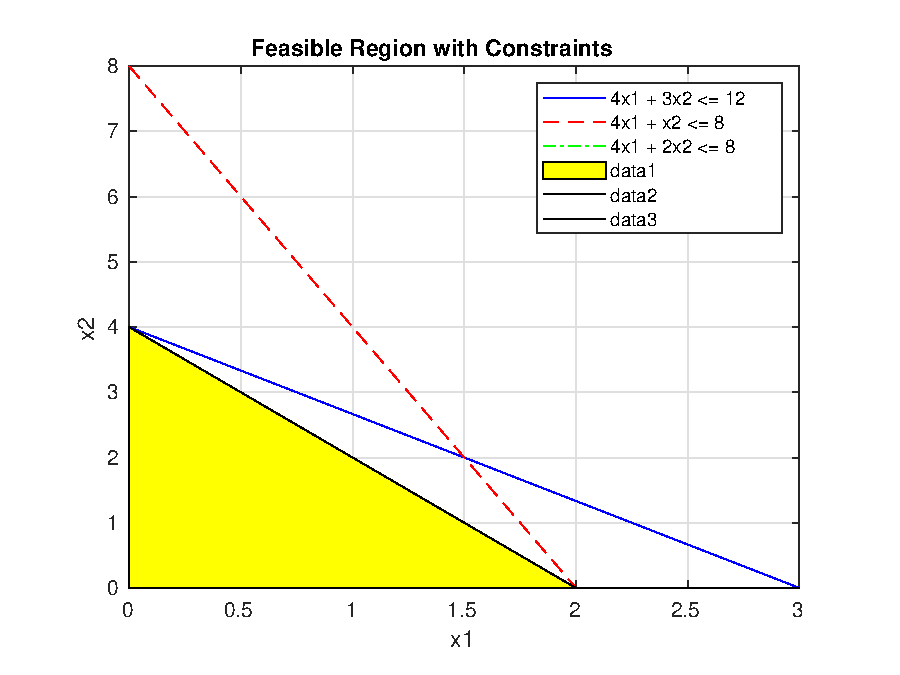
\includegraphics[width=\textwidth, trim={0cm 0cm 0cm 0cm}]{./figures/ex4-2-plot.eps}
\end{figure}




\section{Quality of the Code \& Report [15 points]}

Each project sums up to 100 points, out of which 15 points are dedicated to the general quality of your written report and of the code submitted. Your report should be a coherent document. If there are theoretical questions, explain and justify your answers. If you made a particular choice in your implementation that might be out of the ordinary, please explain it in the report. The code you submit should be self-contained and executable. It should include the set-up for all the results that you obtained and listed in your report. Furthermore, it should be readable and include comments explaining the more complicated steps.


\end{document}
